% TO DO LIST Background
% LDA
% Strike a match
% Pyramid score
% Sequential pattern mining
% abstract code summary tree bring from later chapter and enhance
% Background related works for committee

\label{chapter:background}

In this chapter, we briefly discuss relevant terms, topics and techniques helpful to this thesis. In Section \ref{background:call_graph}, we elaborate terms relevant to a call graph. We then present an  abstract code summary tree in Section \ref{background:cct}. In Section \ref{background:motive}, we provide an abstract code summary tree for a sample calculator program using our system. In Section \ref{background:techniques}, we have elaborated different techniques and algorithms used in the thesis. 

\section{Call graph}
\label{background:call_graph}
A \emph{call graph} is a control flow graph of a program showing calling relationships between functions. Each node of the graph represents a function and each edge $(a, b)$ represent calling relationship where function $a$ calls function $b$. Figure \ref{fig:bg_call_graph} shows a simple call graph with six nodes indicating functions and six edges indicating calling relationships. Call graphs can be two type. One type is static call graph. A static call graph contains all the possible program execution scenarios. To generate a static call graph, source code of the program is analyzed to find the relationships. A dynamic call graph represents one program run scenario. Therefore, a dynamic call graph is exact and limited to the scenarios used to generate the graph. To generate a dynamic call graph, logger or profiler is applied which generates call graph during run-time of the program.

\begin{figure}[h]	
	\centering
	\begin{subfigure}[h]{3in}
	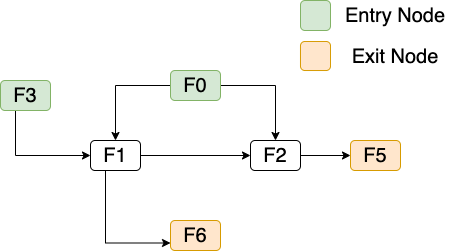
\includegraphics[width=3in]{figures/background/call graph.png}
	\caption{A sample call graph}\label{fig:bg_call_graph}		
	\end{subfigure}
	\quad
	\begin{subfigure}[h]{3in}
		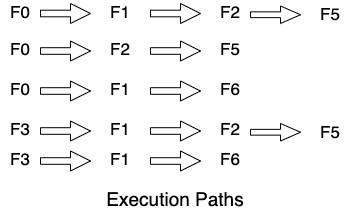
\includegraphics[width=3in]{figures/background/execution_paths.png}
		\caption{All execution paths from the call graph}\label{fig:bg_execution_path}
	\end{subfigure}
	\caption{Call graph with entry node, exit node and execution paths}\label{fig:1}
\end{figure}

An \emph{entry node} for a call graph is the nodes which number of incoming degree is zero. In Figure \ref{fig:bg_call_graph}, the call graph has two entry nodes \emph{F0, F3}. No other nodes call the functions or nodes \emph{F0, F3}. That means program execution can start from this nodes.

An \emph{exit node} for a call graph is the nodes which number of outgoing degree is zero. In Figure \ref{fig:bg_call_graph}, the call graph has two exit nodes \emph{F0, F3}. The exit nodes \emph{F0, F3} do not call any other functions or nodes. That means program execution will end when we come to this node.


The \emph{execution paths} of a call graph are the all possible program execution scenarios. A program execution scenario consist of a function call sequence starting from a \emph{entry node} and ending to a \emph{exit node} of the call graph. In Figure \ref{fig:bg_execution_path}, all the execution paths from the call graph of Figure \ref{fig:bg_call_graph} are listed. First node of the execution paths are the Entry nodes which is defined above. Similarly, Last node of the execution paths are the Exit nodes. 




\section{Abstract code summary tree}
\label{background:cct}
In this thesis, we introduce a term called abstract code summary tree (ACST). ACST is a tree where each leaf node is attached to an execution paths extracted from call graph of a software. The parent nodes of the leaf nodes are grouping of similar execution paths (leaf nodes). We call this intermediate nodes as abstraction node as they abstract similar execution scenarios. Each abstraction node has three properties which are title, text summary and execution patterns. 

\begin{figure}[h]
  \centering
  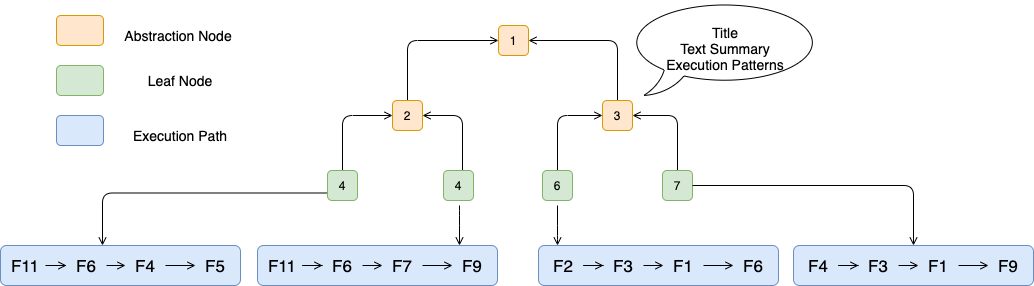
\includegraphics[width=\columnwidth]{figures/background/cct.png}
  \caption{An abstract code summary tree with its different components }
  \label{background:cct}
\end{figure}
In Figure \ref{background:cct}, we present a ACST where \emph{4, 5, 6, 7} nodes are leaf node which are attached to execution paths. Nodes \emph{1, 2, 3} are abstraction nodes which are grouping of the leaf nodes. Each abstraction nodes has number of execution paths and we use different information from those execution paths to generate concepts for them. Node 3 has two execution paths which belong to node 6 and 7. Like all other abstraction nodes Node 3 will have title, text summary and execution patterns. The title of Node 3 will be generated using different information retrieval techniques on method signatures. Next, The text summary of Node 3 will be generate by summarizing comments of the methods which belong to the execution paths of Node 3. The execution patterns of the Node 3 will be generated by finding frequent patterns on the execution paths of Node 3.

\section{Motivational Example}
\label{background:motive}
To demonstrate how a software system's hierarchical abstraction will work, we have created a sample Calculator program. The program takes two numbers as input, validates the inputs, and prompts the user to input which operations they want to perform. Later, according to the input, addition, subtraction, multiplication, division can be performed. This is a brief functionality of the calculator program. We have provided the source code of the Calculator program in appendix \ref{appendix:calculator}.

In Figure \ref{fig:motivation} we have presented the hierarchical abstraction of the Calculator program. From the figure, we can see our Calculator program has six execution paths. Their node number is from 0-5. 

\begin{figure}[h]
  \centering
  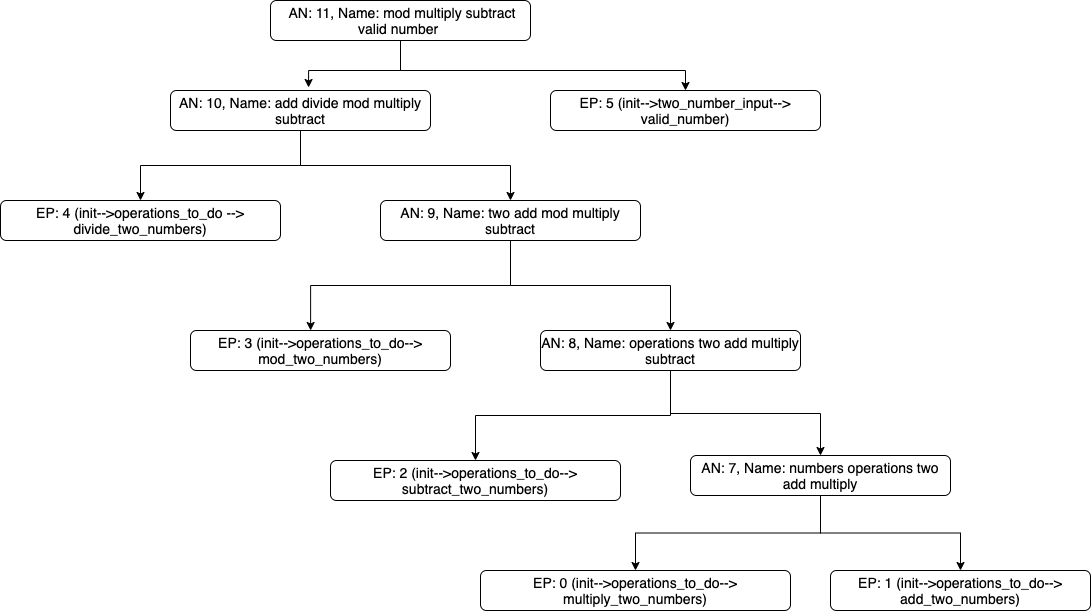
\includegraphics[width=\columnwidth]{figures/hla2/hla2_motivation.png}
  \caption{An abstract code summary of the calculator program (EP means Execution path or leaf node and AN means Abstraction Node)}~\label{fig:motivation}
\end{figure}

\textbf{Constructing the abstract code summary.} To generate the tree shown in Figure \ref{fig:motivation}, the following steps are followed.

\begin{enumerate}
    \item To get the caller-callee relationship from the source code of Calculator program, we use static source code analyzer.
    \item We construct static call graph from the extracted relationships of \emph{Calculator.py} program. 
    \item From the call graph, possible execution scenarios are generated  which are the execution paths shown in Figure \ref{fig:motivation} (EP 0 - 5).
    \item Similarity score for each pair of execution paths are calculated which is used by the clustering algorithm to group the execution paths. As EP 0, 1, ...., 4 all have three common functions, the similarity measure between them  will be same.  
    \item Clustering algorithm starts grouping the execution paths by taking the most similar two first. In Figure \ref{fig:motivation}, we see that EP 0, 1 are grouped together as abstraction node (AN) 7.
    \item As AN 7 have EP 0, 1, we use information retrieval techniques on all the terms in functions names of EP 0, 1 to label the AN 7. 
    \item Although keywords are helpful for hint, having a text description and frequent execution patterns for each abstraction node increases comprehension. In Table \ref{table:node_summary_patterns}, we presented node summary and execution patterns for AN 10, 11. 
    
\end{enumerate}



\begin{table*}[h]
\caption{Abstraction Nodes with summary and execution patterns}
    \centering
    \begin{tabular}{ |l | p{5cm} | p{10cm} | } 
 \hline
 AN & Node Summary & Execution Patterns \\ 
 \hline
 11 & This function multiply two numbers. This function mod two numbers. This function subtract two numbers.  &  \bullet init \rightarrow two\_number\_input \rightarrow valid\_number. 
 \bullet init \rightarrow operations\_to\_do \rightarrow add\_two\_numbers. 
 \bullet init \rightarrow operations\_to\_do \rightarrow divide\_two\_numbers. 
\bullet init \rightarrow operations\_to\_do \rightarrow mod\_two\_numbers. 
 \bullet init \rightarrow operations\_to\_do \rightarrow multiply\_two\_numbers. 
 \bullet init \rightarrow operations\_to\_do \rightarrow subtract\_two\_numbers. \\ 
10 & This function mod two numbers. This function divide two numbers. This function subtract two numbers. & 
\bullet init \rightarrow operations\_to\_do \rightarrow add\_two\_numbers. 
\bullet init \rightarrow operations\_to\_do \rightarrow divide\_two\_numbers. 
\bullet init \rightarrow operations\_to\_do \rightarrow mod\_two\_numbers. 
\bullet init \rightarrow operations\_to\_do \rightarrow multiply\_two\_numbers. 
\bullet init \rightarrow operations\_to\_do \rightarrow subtract\_two\_numbers. 
\\ 
 \hline
\end{tabular}
    \label{table:node_summary_patterns}
\end{table*}



\textbf{Exploring the abstract code summary.}
\begin{itemize}
    \item Execution path 0 and 1 represent the functionality of multiply two numbers and adding two numbers, respectively. For these two clusters, add and multiply is the two different job they are doing. Other functions of the two paths are similar. So, the abstraction of these two execution paths is abstractioin node 7. Five keywords are picked as the abstraction of execution paths 0 and 1. From the keywords of node 7, it is clear that descendent nodes do addition and multiply on two numbers.
    \item Next, for node 10, we can see the keywords are add, divide, mod, multiply, and subtract. These five keywords indicate that the descendant nodes of 10 do these numerical operations. If we observe the five execution paths (EP 0 - 4), we find that they perform add, delete, mod, multiply operation on two input numbers. We can see that the five keywords of node 10 summarize the functionality of its descendants.
    \item Similarly, for node 11, the keywords are mod, multiply, subtract, valid, and number. We can see the right child node (node 5) of node 11 input two numbers and then validates it. Left descendants of node 11 perform numerical operations. So, the summary of node 11 contains three words relevant to operation and two for input validation.
\end{itemize}
   From our understanding, we can see that this is an almost human level summary for node 10. The summary presented in Figure \ref{fig:motivation} is generated using Tfidf score on words in method name. 

\section{ Techniques \& Algorithms}
\label{background:techniques}
\subsection{TFIDF}
TFIDF is weight based statistical information retrieval technique. It tries to find important terms to a specific document by analyzing collection of documents. TFIDF is popular for document classification, search engine ranking and text mining\footnote{https://en.wikipedia.org/wiki/Tf–idf}. TFIDF ranks terms by term frequency-inverse document frequency score. Term frequency is count of a term in a document. Term frequency is biased towards common terms which mostly irrelevant to the document. 

\begin{equation}
    tf (W_x, D_x) = f_{W_x,D_x}
    \label{eq:tf_background}
\end{equation}
\begin{equation}
    idf(W_x) = \log(\frac{n}{df(W_x)})+1
    \label{eq:idf_background}
\end{equation}
\begin{equation}
    tf-idf(W_x, D_x) = tf(W_x,D_x) * idf(W_x)
    \label{eq:TFIDF_background}
\end{equation}


Jones \cite{jones1972statistical} introduced inverse document frequency which penalties common terms by counting their occurrence across the corpus. Let, $D = \{D_1, D_2, ..., D_n\}$ is a collection of documents and $W = \{W_1, W_2, ....., W_n\}$ is unique terms in the collection of documents. Now, to calculate term frequency for term $W_x$ in document $D_x$, we have to count frequency of term $W_x$ in  document $D_x$ which is required to calculate term frequency according to equation \ref{eq:tf_background}. In addition, we have to count the number of documents has term $W_x$ which is used to calculate inverse document frequency using equation \ref{eq:idf_background}. In equation \ref{eq:idf_background}, $n$ is the number of documents in the corpus and $df(W_x)$ is the number of documents which contain term $W_x$. Equation \ref{eq:TFIDF_background}, multiplies term frequency and inverse document frequency to reward significant terms and penalize common terms. 



\subsection{LSI}
Latent semantic indexing focuses on information retrieval based on semantic similarity between words where the previous techniques focus on matching words in query with words of documents. The semantic concept used in LSI assumes semantically similar words appear together. Information retrieval techniques which matches words suffer two limitations. They are \emph{synonymy} and \emph{polysemy}. \emph{synonymy} is the issue where same object is described by different words depending on needs, knowledge and linguistic habits. On the other hand, \emph{polysemy} is referred to the fact that words have multiple distinct meaning in different context. LSI, first, starts with Term-Document matrix where all terms are presented in the row and documents in the column. Table \ref{tb:LSI_term_document} shows an example of Term-Document matrix. 

\begin{table}[h]
    \centering
    \caption{Sample Term-Document matrix}
 \begin{tabular}{|c|c|c|c|c|c|c|}
    \hline
    
        & ship & boat & ocean & voyage & trip   \\
        \hline
        Document 1 & 1 & 0 & 1 & 0 & 0  \\
        Document 2 & 0 & 1 & 0 & 1 & 0    \\
        Document 3 & 1 & 0 & 0 & 1 & 1  \\
    \hline
    \end{tabular}
    
    \label{tb:LSI_term_document}
\end{table}


Term-Document matrix is projected to lower number of dimensions by Single Value Decomposition (SVD) method. The reduced matrix by SVD is approximation of the term-document matrix which is a representation of the semantic similarity between words in documents. If we need to find similarity between a query, the query is converted to similar representation and compared to find relevant documents. By using this technique, LSI can detect semantic similarity although the terms are different.   

% \subsection{LDA}

\subsection{Jaccard Distance}
Jaccard Distance can measure similarity between two sequences according to equation \ref{eq:jaccard}. For example, we have two execution path $E_i$ and $E_j$ and they have set of function names $F_i$ and $F_j$ respectively. Therefore, similarity between $E_i$ and $E_j$ can be measured by equation \ref{eq:jaccard}. 
\begin{equation}
\label{eq:jaccard_similar}
    JD\_similar(E_i, E_j) =  \frac{F_i \bigcap F_j}{F_i \bigcup F_j}
\end{equation}

\begin{equation}
\label{eq:jaccard_dissimilar}
    JD\_dissimilar(E_i, E_j) =  1 - \frac{F_i \bigcap F_j}{F_i \bigcup F_j}
\end{equation}
If $E_i$ and $E_j$ are very similar, according to equation \ref{eq:jaccard_similar} similarity score will be near 1 and vice-versa. Clustering algorithm merges those two clusters which distance measures are minimum. Equation \ref{eq:jaccard_dissimilar} subtract Jaccard Distance by 1 to get desire dissimilarity measure for clustering algorithms.

\subsection{Agglomerative Hierarchical Clustering}
Clustering algorithms are popular in many data mining, unsupervised machine learning and pattern recognition applications. Clustering algorithm try to group similar observations together to find significant patterns in the observations. Hierarchical clustering can be done in two ways. One is bottom-up (agglomerative) and another is top-down (devisive). For Devisive clustering, all observations starts in a single cluster and divided into different clusters using heuristics. Agglomerative clustering starts by considering observations as individual clusters and then group them until all observations end-up in the same cluster.

\begin{figure*}[h]
  \centering
  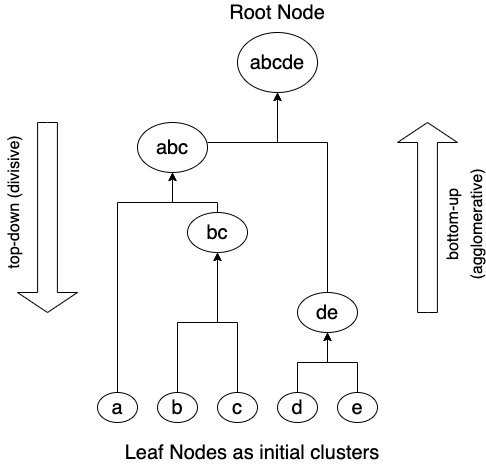
\includegraphics[width=0.5\columnwidth, height=0.5\columnwidth]{figures/background/agglomerative_clustering.png}
  \caption{Agglomerative and Divisive clustering algorithm with a sample cluster forest}~\label{fig:agglomerative_clustering}
\end{figure*}
In Figure \ref{fig:agglomerative_clustering}, a visualization of how agglomerative and divisive clustering algorithm works are presented. Lets assume there are five observations \emph{a, b, c, d, e} and we have similarity score between all the pairs of the observations. First, we can see five observations are treated as five clusters. From the similarity score we found that clusters \emph{d and e} are most similar. Therefore, we group cluster \emph{d and e} together as a new cluster \emph{de}. Now, in the cluster forest we have four clusters. In the next step, cluster b and c are the most similar. So, agglomerative clustering algorithm will group cluster b and c as a new cluster \emph{bc}. The agglomerative clustering will continue to merge clusters together until there is only one cluster in the cluster forest. For this example, the final cluster \emph{(abcde)} consists of all the initial clusters. 

\subsection{Text Rank}
Mihalcea \cite{mihalcea2004textrank} proposed graph based ranking algorithm inspired by PageRank algorithm to rank entities in natural language. Two of the significant application of TextRank are keyword extraction and sentence extraction. Sentence extraction can be formulated to generate summary of natural language text. To generate summary of a  text, first, sentences are split as they are the unit for TextRank algorithm. Next, sentences are converted to word embedding vectors. In the next step, similarity matrix is computed from embedding vectors. Then, a graph is created where vertices are sentences and edges represent similarity scores between sentences\footnote{https://www.analyticsvidhya.com/blog/2018/11/introduction-text-summarization-textrank-python/}. Similarity scores are used to extract top ranked sentences according to equation \ref{eq:textrank}.

\begin{equation}
\label{eq:textrank}
    WS(V_i) = (1 - d) + d * \sum_{V_j\epsilon IN(V_i) } \frac{w_{ji}}{\sum_{V_k \epsilon Out(V_j)} w_{jk}}  WS(V_j)
\end{equation}

Let, $ G = (V, E)$ is a directed graph where V is the collection of vertices and E is the collection of edges. $In(V_i)$ is the set of vertices which points to vertex $V_i$. Similarly, $Out(V_j)$ is the set of vertices which vertex $V_j$ points to. The similarity score between vertex $V_i$ and $V_j$ is represented by $w_{ji}$. 

% \section{Pyramid Score}

% \section{Sequential Pattern Mining}






